\section{Conluzii}
Prover9 și Mace4 pot fi folosite pentru a rezolva diferite tipuri de puzzle-uri și jocuri sociale. În general, acești demonstratori de teoreme funcționează luând un set de ipoteze logice și o formulă de obiectiv ca intrare și apoi încercând să găsească o soluție care să satisfacă ipotezele și obiectivul.\newline\newline
Pentru a utiliza Prover9 și Mace4 pentru puzzle-uri și jocuri sociale, primul pas este să exprimăm regulile și constrângerile puzzle-ului sau jocului ca formule logice.\newline\newline
Odată ce am exprimat regulile și constrângerile puzzle-ului sau jocului ca formule logice, putem folosi Prover9 sau Mace4 pentru a găsi o soluție care să satisfacă aceste formule.
\newline\newline

\begin{figure}[h]
    \centering
    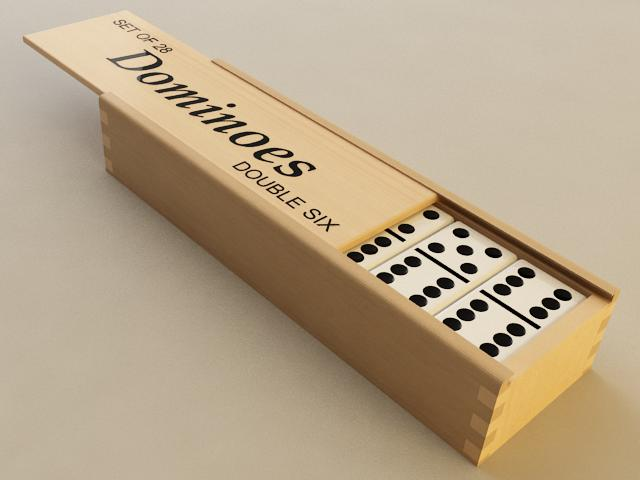
\includegraphics[width5cm]{text/images/pic10.jpg}\\

\end{figure}

